\documentclass{rapport}
\usepackage[utf8]{inputenc}

\usepackage{pifont} % Pour les symboles appelés par la macro \ding
\usepackage{url} % Comme son nom l'indique, pour les url...

\usetikzlibrary{positioning} % Bibliothèque tikz pour positionner des nœuds relativement à d'autres

\usepackage[colorlinks, citecolor=red!60!green, linkcolor=blue!60!green, urlcolor=magenta]{hyperref} % Pour que les liens soient cliquables. Les options permettent de mettre les liens en couleur.

\usepackage{algorithm}
\usepackage{algo}
\usepackage{colorationSyntaxique}


% Pour un rapport en français 
\usepackage[francais]{babel} % Commenter pour un rapport en anglais
\renewcommand\bibsection{\section*{Bibliographie}} % Commenter pour un rapport en anglais

% \englishTitlePage % Décommenter pour une page de titre en anglais


\pagestyle{fancy}
\renewcommand{\sectionmark}[1]{\markboth{\thesection.\ #1}{}}
\fancyfoot{}

\fancyhead[LE]{\textsl{\leftmark}}
\fancyhead[RE, LO]{\textbf{\thepage}}
\fancyhead[RO]{\textsl{\rightmark}}

\def\Latex{\LaTeX\xspace}
\def\etc{\textit{etc.}\xspace}



\title{Travaux Pratiques sur la Hiérarchie Mémoire }
\author{Francois Flandin}
\supervisor{Pr Sid Touati}
\date{Premier semestre de l'année 2024-2025}

% \universityname{Université Côte d'Azur} % Nom de l'université.
\type{TP} % Type de document
% \formation{Master Informatique} % Nom de la formation

% Retrouver les autres options possibles dans le document rapport.pdf

\begin{document}

    \maketitle


    \clearpage
    \tableofcontents

    \clearpage

    \section{Introduction}
    Ce rapport présente le travail réalisé dans le cadre d’un TP visant à explorer les performances de la hiérarchie mémoire d’un processeur. L’objectif était d’analyser le comportement des caches et de la mémoire centrale à travers des tests pratiques, tout en utilisant des outils simples et adaptés.

    En partant des caractéristiques techniques du processeur de test, on a mis en place des expériences pour mesurer les temps d’accès à la mémoire et la bande passante. Les données obtenues ont ensuite été analysées pour mieux comprendre les mécanismes en jeu, comme le prefetch matériel ou les optimisations logicielles.
    
    Ce document retrace les étapes principales de cette étude, les méthodes utilisées, et les enseignements tirés des résultats.

    \section*{Environnement Expérimental}
    \subsection*{Micro-Architecture}
    Dans cette partie sera detaillée la micro-architecture de la machine de tests.
    \newline\newline
    \textbf{Nom de modèle :} 11th Gen Intel(R) Core(TM) i5-1135G7 @ 2.40GHz
    \newline
    \textbf{Taille des adresses :} 39 bits physical, 48 bits virtual
    \newline
    \textbf{Coeurs physiques :} 4
    \newline
    \textbf{Taille de ligne de cache :} 64 octets

    \begin{table}[h!]
        \centering
        \begin{tabular}{|l|c|c|c|c|}
            \hline
            \multicolumn{5}{|c|}{Graphical Topology} \\
            \hline
            Coeurs & \enspace0\enspace\enspace4 &\enspace1\enspace\enspace5 &\enspace2\enspace\enspace6 &\enspace3\enspace\enspace7 \\
            \hline
            Cache L1 & \enspace48 kB &\enspace48 kB &\enspace48 kB &\enspace48 kB \\
            \hline
            Cache L2 & 1MB & 1MB & 1MB & 1MB \\
            \hline
            Cache L3 & \multicolumn{4}{|c|}{8 MB} \\
            \hline
        \end{tabular}
        \caption{Topologie de la machine de tests}
        \label{tab:graph_characteristics}
    \end{table}
    
    
    \subsection*{Environnement Logiciel}
    Dans cette partie sera détaillée la partie logiciel de la machine de test, les fichiers scripts pour changer entre machine allégée et machine classique sont fournis dans l'archive.
    \newline\newline
    \textbf{Distribution :} Fedora v40 WorkStation
    \newline
    \textbf{Compilateur utilisé :} \texttt{gcc} version 14.2.1 20240912 avec option \texttt{-O0}
    \newline
    \textbf{Outil de mesure des temps d'exécution :} fonction \texttt{gettimeofday} de C de la librairie \texttt{sys/time.h}.

    \section*{Configuration expérimentale}
    \subsection*{Processus en activité}
    \begin{verbatim}
    > ps -x
    PID TTY      STAT   TIME COMMAND
   1263 ?        Ss     0:00 /usr/lib/systemd/systemd --user
   1265 ?        S      0:00 (sd-pam)
   1284 tty1     Ss     0:00 -zsh
   1898 tty1     R+     0:00 ps -x
    \end{verbatim}
    Voici ce que font les processus en cours d'exécution.
    \newline\newline
    \textbf{systemd :} C'est un système d'initialisation et de gestion de services sous Linux, conçu pour démarrer, arrêter et superviser les processus, tout en offrant une gestion centralisée des sessions et des ressources.
    \newline
    \textbf{sd-pam :} \textit{systemd-PAM} C'est un utilitaire de \texttt{systemd} pour gérer les sessions.
    \newline
    \textbf{zsh :} C'est le shell qui est lancé pour exécuter les commandes.
    \newline
    \textbf{ps -x :} C'est la commande qui a été lancée pour voir les processus.
    
    \subsection*{Méthodologie de récolte des données expérimentales}
    Pour la premiere partie, après avoir mesuré les differents temps moyen d'accès, le programme C l'affiche sur la sortie standard afin d'exécuter la commande \texttt{./benchmark > bench.csv} pour rassembler toutes les sorties dans un fichier. De plus, le programme affiche les données sous format \texttt{csv} pour permettre un meilleur traitement avec le logiciel \texttt{gnuplot}.\newline
    Pour la deuxieme partie, le programme affiche simplement le résultat sur la sortie standard, il nous reste donc juste a récupérer le résultat avec un \texttt{./benchmark > res.data}, exécuté 4 fois ou plus avec une boucle \texttt{for}.\newline
    Pour la dernière partie, l'outil utilisé se charge lui-même de mettre les résultats dans des fichiers \texttt{.data}, que l'on pourra plot avec les fichiers \texttt{.gp} et \texttt{gnuplot}.

    \clearpage
    
    \section{Tester les performances de la hiérarchie mémoire d’un CPU avec un micro-benchmark séquentiel}
    \begin{figure}[H]
    \centering
    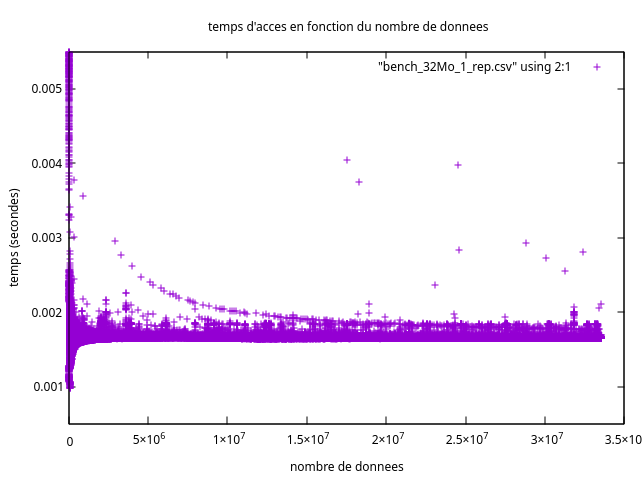
\includegraphics[width=1\textwidth]{../exercice_1/resultats/resultats.benchmark-1rep-32Mo.png}
    \caption{Résultats du benchmark avec un tableau de taille 32Mo et une répétition par accès.}
    \label{fig:image1}
    \end{figure}
    \begin{figure}[H]
    \centering
    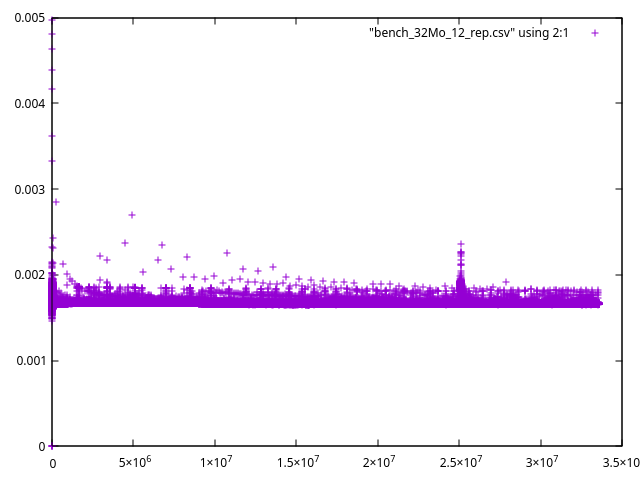
\includegraphics[width=1\textwidth]{../exercice_1/resultats/resultats.benchmark-12rep-32Mo.png}
    \caption{Résultats du benchmark avec un tableau de taille 32Mo et 12 répétitions par accès.}
    \label{fig:image2}
    \end{figure}

    Ce que l'on remarque sur ces graphiques c'est qu'aucun "palier" n'apparaît, cela pourraît être dû au prefetch matériel, on remarque même que les temps d'accès dimininuent avec le temps.\newline
    On observe aussi qu'avec 12 répétitions, les temps d'accès sont plus stables.

    \clearpage
    
    \section{Evaluation de la bande passante entre le processeur et la mémoire centrale.}
    Dans cette partie sera expliqué comment à été évaluée la bande passante entre le processeur et la mémoire centrale, une brève analyse des résultats sera aussi proposée. \newline
    \subsection{Méthode}
    Pour calculer la bande passante entre le processeur et la mémoire centrale, il est d'abord nécessaire de calculer le temps moyen d'accès a la mémoire, et de connaître un peu notre machine. Les données qui sont importantes a connaître sont, la taille du cache L3 ainsi que la taille de la ligne de cache. Ils vont servir a déterminer la taille du tableau ainsi que la taille du pas pour éviter qu'une donnée soit préchargée en mémoire, on doit donc prendre 2 fois la taille du cache L3 et un pas suffisament grand pour être sûr de dépasser le prefetch matériel ainsi que le préchargement des données dans un cache. \newline
    La taille du cache L3 de la machine de test est de 8Mo, on a donc $(2 * 8 * 1024 * 1024)/sizeof(int)$, ce qui donne 4194304 élements, quand à la taille du pas, on choisira un pas très grand, 4 fois et 8 fois la taille de la ligne de cache, réalisés avec des \texttt{bit shift} pour s'assurer qu'aucune donnée ne soit préchargée, on remarquera que plus on augmente le pas, plus le temps d'accès moyen à la mémoire augmente.
    \subsection{Résultats}
    \begin{table}[H]
    \centering
    \begin{tabular}{c|c|c}
    Multiplicateur de pas & Temps d'acces moyen (en ns) & Bande passante (en Mo/s) \\
    \hline
     4 & 62,49237075 & 985,63519275 \\
     8 & 116,783142 & 563,27429225 \\
    \end{tabular}
    \caption{Résultats moyens des tests de performance mémoire sur 4 exécutions du benchmark.}
    \end{table}
    De plus, si on regarde les résultats inclus dans l'archive, on remarque que plus on effectue d'exécution consécutives, plus le temps d'accès a la mémoire diminue et le débit augmente, cela pourrait venir du système d'exploitation qui optimiserait par lui-même, ou en augmentant la vitesse du processeur.

    \clearpage

    \section{Etude de l'outil Calibrator}

    Les résultats du benchmark réalisé avec \texttt{Calibrator} sont laissés dans l'archive, l'objectif ici est de comprendre pourquoi cet outil est mieux que les benchmarks réalisés précédemment. \newline
    Si on s'en tient a la documentation du logiciel, \texttt{Calibrator} permet de mesurer les différents niveaux de cache, avec pour chaque cache, sa taille, sa taille de ligne de cache, on remarque d'ailleurs sur les résultats que la taille augmente selon le niveau de cache, c'est sans doute une des raisons pour lesquelles on n'observait pas de "palier" au premier benchmark, et aussi la latence d'accès ou d'échec au niveau de cache. \newline
    L'outil permet aussi de mesurer les différents niveaux du \texttt{TLB}, qui est un cache mémoire qui permet de stocker les dernières traductions adresse virtuelle/adresse physique, évitant ainsi d'avoir à les chercher dans la mémoire centrale. Ce qui est une très grande différence avec les benchmarks réalisés plus tôt, qui nous permettaient de calculer uniquement les temps d'accès aux niveaux de cache ainsi que la bande passante entre le processeur et la mémoire centrale. L'analyse des niveaux de TLB viennent avec la mesure de sa capacité, de la taille d'une page mémoire, ainsi que la latence d'échec. \newline
    L'outil peut aussi mesurer la latence d'accès à la mémoire centrale, en additionnant simplement les \textit{latences d'échec} de tous les niveaux de cache.
    Les différences avec les précédents benchmarks ne s'arrête pas là, il y a aussi la façon dont l'outil réalise ses benchmarks, il change plusieurs fois pendant le benchmark la taille du pas, appelée \texttt{stride} en anglais, tandis que sur nos benchmarks, la taille du pas était fixe.


    \section{Conclusion}
    Dans ce travail pratique, les performances de la hiérarchie mémoire d'un processeur ont été étudiées à travers plusieurs tests et mesures. En regardant les temps d’accès moyen et la bande passante, on a pu voir comment des paramètres comme la taille des tableaux et le pas de lecture influencent les résultats. \newline
    Plusieurs détails intéressants en sont sortis, comme premièrement l’absence de "paliers", probablement à cause du prefetch matériel, et une amélioration des performances après plusieurs exécutions, sûrement grâce à des optimisations du système. \newline
    Ces tests montrent à quel point il est important de bien comprendre le fonctionnement des caches et de la mémoire pour optimiser les performances. Cela ouvre aussi la porte à des études plus poussées, sur les effets des réglages du système ou sur les optimisations matérielles par exemple.
    

\end{document}
